\problemname{Youngdiagram}

\begin{figure}[!h]
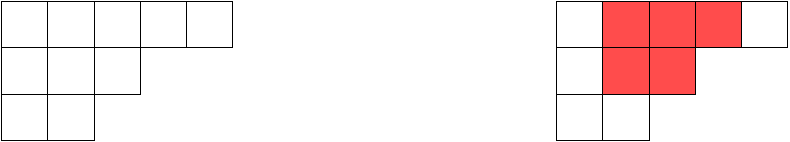
\includegraphics[width=0.98\textwidth]{young}
\caption{Till vänster visas Young-diagrammet som motsvarar partitioneringen 10=5+3+2. Till höger demonstreras att diagrammet för 10=5+3+2 (svarta konturer) kan omsluta diagrammet för 5=3+2 (fyllda rutor). Å andra sidan kan inte diagrammet för 10=5+3+2 omsluta diagrammet för 8=4+4.}
\end{figure}

Ett \emph{Young-diagram} är ett sätt att åskådliggöra en partitionering av ett positivt heltal $n$ i en eller flera heltalstermer:

$$n = m_1 + m_2 + ... + m_k$$

Diagrammet består av $k$ rader med $m_i$ rutor i varje rad (se figuren ovan). Raderna är vänsterjusterade och alltid sorterade i längdordning så att översta raden representerar den största termen o.s.v. En viss rad är alltså antingen kortare än raden ovanför eller lika lång som den. Ibland kan ett Young-diagram \emph{omsluta} ett annat. Vi säger att diagram X kan omsluta diagram Y om det är möjligt att placera diagram Y, utan att rotera eller spegla det, fullständigt inuti diagram X, d.v.s. så att varje ruta i Y sammanfaller med en ruta i X.

Skriv ett program som, givet ett heltal $n$, hittar den partitionering av $n$ vars Young-diagram kan omsluta det största antalet olika Young-diagram.

\section*{Input}
Indatan består av hetalet $n$ ($1 \le n \le 100$).

\section*{Output}
Skriv ut ett heltal: det maximala antalet Young-diagram som något enstaka Young-diagram med $n$ rutorkan omsluta.
Skriv därefter ut en rad med ett eller flera positiva heltal, antalet rutor i varje rad av detta optimala diagram,
med början uppifrån. Om det finns flera optimala diagram kan du ange vilket som helst av dem.

\section*{Poängsättning}
Din lösning kommer att testas på en mängd testfallsgrupper.
För att få poäng för en grupp så måste du klara alla testfall i gruppen.

\noindent
\begin{tabular}{| l | l | p{12cm} |}
  \hline
  \textbf{Grupp} & \textbf{Poäng} & \textbf{Gränser} \\ \hline
  $1$    & $10$       & $n \leq 10$ \\ \hline
  $2$    & $25$       & $n \leq 20$ \\ \hline
  $3$    & $25$       & $n \leq 60$ \\ \hline
  $4$    & $40$       & Inga ytterligare begränsningar. \\ \hline
\end{tabular}
